\chapter{Evaluation}
\label{ch:Evalutation}
In the introduction chapter, the \textit{Research Questions} are presented. The third question is about the elaborated approach and its evaluation.



\vspace{0.5cm}
\par
\begingroup
\leftskip=1cm
\rightskip=1cm

\noindent
\textbf{RQ3: What is the accuracy of the approach? }

\endgroup
\vspace{0.5cm}

\noindent
To tackle this question, a \textit{Goal Quality Metrics Plan } (GQM) is introduced to specify the key aspects of the evaluation. In a word, the elaborated approach is used to identify a set of microservice candidates which is compared to two reference sets of microservices. \\
In the following, a \textit{GQM Plan} is introduced to specify what exactly needs to be evaluated. Also, metrics to measure the results of the comparison are introduced. Second to last, the two reference sets are illustrated before the actual results of the approach are finally depicted.




\section{GQM Plan}
\label{sec:Evaluation:GQM}
Basili et al. originally proposed the \textit{GQM Plan} (Goal Quality and Metrics) as a paradigm in software engineering but it is further extended to other engineering disciplines \cite{BasiliGQM}. Based on a precise and structured procedure, the paradigm enables a high traceability and 
assessment of the engineering process. The main purpose is to specify the goals for a project, illustrate the data to define these goals and provide an environment to interpret the collected data. In the case of this thesis, the \textit{GQM Plan} is used to clarify the desired intention of the evaluation in order to prevent unnecessary metrics and measurements and consequently reduce the expenditure of work. \\
The \textit{GQM Plan} is a Top-Down approach and divided in three fundamental steps that precede the measurement and evaluation of results. First, the goal of the evaluation is defined on a conceptual level. Seconds, questions are delineated to achieve the specific goal. Finally, to answer the questions in a measurable way, metrics have to be defined that are associated with the questions. \\
In the following, the \textit{GQM Plan} for this the consecutive evaluation is illustrated:

\begin{itemize}
	\item \textbf{G1:} Determine the accuracy of the approach
	\item \textbf{G1.Q1:} What is the \textit{Precision and Recall} of the identified microservices compared to the reference amount?
	\item \textbf{G1.Q1.M1:}  Precision and Recall
	\item WAS WAR HIER NOHCMAL MIT DEN ZYKLISCHEN ABHÄNGIGKEITEN
\end{itemize}




\section{Metrics}
\label{sec:Evaluation:Metrics}
%TODO Weitere Metriken als nur precision recall
Using metrics is mandatory to measure the quality of the elaborated approach. In this case, it is required to choose a metric to classify a set of instances, namely microservices, regarding their relevance. Two reference sets are available as further depicted in Sec.\ref{sec:Evaluation:ReferenceSets}. \\
A metric that is capable to measure the relevance of a set of instances compared to a reference set is \textit{Precision and Recall}. In subsequent, the proposed metric is briefly presented.

\subsection{Precision and Recall}
\label{sec:Evaluation:Metrics:sPrecRecall}
\textit{Precision and Recall} is a classification metric that measures the relevance of retrievable items with respect to a reference set \cite{PrecisionRecall}. Commonly, two distinctions for items in the reference set are made: First, Retrieved or not Retrieved. More precisely, an item is retrieved if it is part of the selected items and vice versa. Secondly, Relevant or Not Relevant. As a result, all retrievable items belong to one and only one of four cells in the following matrix:


\begin{table}[!h]
	\centering
	\begin{tabular}{|l||l|l|l|}
		\hline
		& Relevant & Not Relevant & Sum \\ \hline
		Retrieved     &     $N_{ret\cap rel}$     &     $N_{ret\cap \overline{rel}}$            &     $N_{ret}$  \\ \hline
		Not Retrieved &      $N_{\overline{ret}\cap rel}$      &      $N_{\overline{ret}\cap \overline{rel}}$          &    $N_{\overline{ret}}$   \\\hline
		Sum           &         $N_{rel}$   &      $N_{\overline{rel}}$          &    $N_{total}$   \\ \hline
		
	\end{tabular}
\caption{Retrieval Matrix, Source: \cite{PrecisionRecall}}
    \label{tab:PrecRecall}
    
\end{table}


\noindent
\textbf{Recall} describes the completeness of the retrieval. In other words, how many relevant items are selected in regard to all possible relevant items.

\begin{centering}
	\vspace{1cm}
	
	$Recall=\dfrac{N_{ret\cap rel}}{ N_{rel} }  $
	
	\vspace{1cm}
\end{centering} 

\noindent
\textbf{Precision} illustrates the purity of the retrieval because it puts into proportion the number of retrieved relevant items and the number of all retrieved items.

\begin{centering}
	\vspace{1cm}
	
	$Precision=\dfrac{N_{ret\cap rel}}{ N_{ret} }  $
	
	\vspace{1cm}
\end{centering} 

 
\noindent
It is important to notice that $N_{\overline{ret}}$ and $N_{\overline{rel}}$ are not part of the formulas. With that in mind, it is possible to apply \textit{Precision and Recall} to the prevalent evaluation scenario. With respect to Table \ref{tab:PrecRecall}, the reference set that is used forms the relevant items, or $N_{rel}$. Accordingly, the set of microservices identified by the proposed approach constitutes the retrieved items, or $N_{ret}$. The remaining part which are the non-relevant and non-retrieved items ($N_{\overline{ret}\cap \overline{rel}}$) are to be unimportant. The following list draws the analogy between Table \ref{tab:PrecRecall} and the predominant evaluation scenario:
\begin{itemize}
	\item \textbf{True Positives:}  $N_{ret\cap rel}$ , identified microservices that have a similar partner in the reference set
	\item  \textbf{False Positives:}  $N_{ret\cap \overline{rel}}$, identified microservices that do not have a similar partner in the reference set
	\item \textbf{False Negatives}:  $N_{\overline{ret}\cap rel}$, microservices in the reference set that have not been discovered by the proposed approach
	\item \textbf{True Negatives}: $N_{\overline{ret}\cap \overline{rel}}$, microservices that are neither discovered by the approach, nor part of the reference set \footnote{Note, that this amount consists of all imaginable microservices and is therefore an infinite set. As it is not used to calculate either of the metrics, it is negligible. }
	
\end{itemize}

\begin{figure}[!h]
	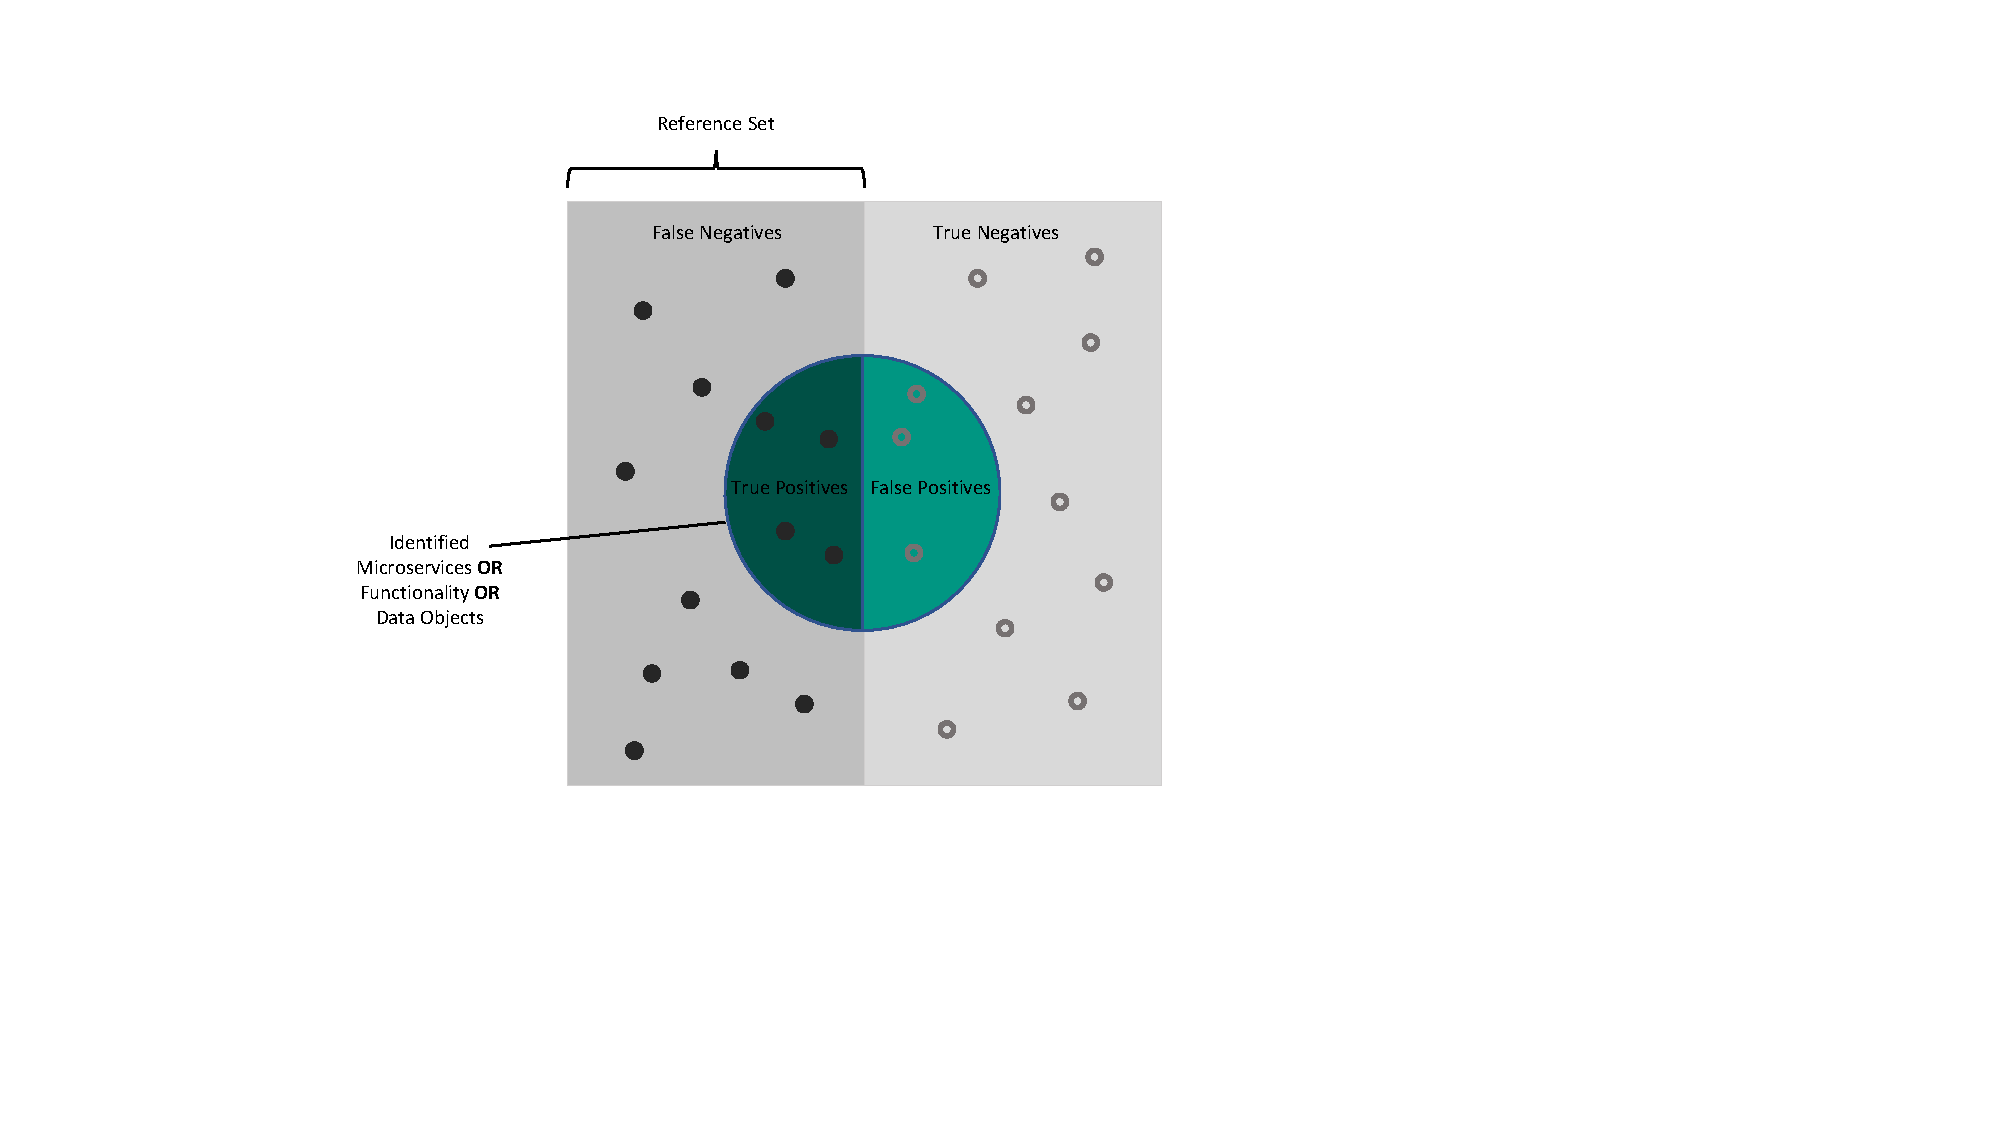
\includegraphics[ trim={7cm 5.5cm 8cm 0.5cm}, scale =1]{img/PrecisionRecall.pdf}
	\caption{Precision and Recall for Microservices}
	\label{fig:PrecisionRecall}
\end{figure}




\subsection{Some more Metrics if necessary}
//Hier noch erklären 



\section{Reference Sets}
\label{sec:Evaluation:ReferenceSets}
To evaluate the approach, the identified set of microservices (cf. Sec.\ref{sec:Evalutation:Results}) is compared to two alternative decompositions of the case study: First, a decomposition proposed in the paper \textit{Identifying Microservices Using Functional Decomposition} \cite{FunctionalDecompositionHeinrich} and second, a set of microservices which we manually identified. \\



\subsection{Reference Set 1: Functional Decomposition Approach}
\textit{Identifying Microservices Using Functional Decomposition} \cite{FunctionalDecompositionHeinrich} is a systematic approach to find a appropriate partition of a system into microservices. This paper emerged as a result of the collaboration of the Academic College Tel-Aviv Yafo, the Karlsruhe Institute of Technology and the Southwest University China and uses CoCoME as demonstrator as well.\\
As depicted in Sec.\ref{sec:stateOfTheArt:approaches}, Tyszberowicz et al. utilize the Use Case specifications of CoCoME \cite{CoCoMEOld} as input for their decomposition approach. Several external tools are used to extract verbs an nouns from the use cases that serve as \textit{system operations} and \textit{state variables}. Irrelevant noun, verbs and synonyms are eliminated via brainstorming. The relationships between the aforementioned concepts are stored in a relation table. A relation exists, if a \textit{system operation} reads or updates a \textit{state variable}. Thereupon, the relation table is visualized as a weighted graph, which enables to identify clusters of dense relationships. Each cluster serves as a microservice candidate.\\
As mentioned in Sec.\ref{sec:stateOfTheArt:comparison}, the compulsory and non-trivial revision of nouns and verbs to eliminate synonyms etc. is a substantial disadvantage. However, the evaluation results in Tyszberowicz's approach demonstrate, that the identified microservices are good candidates for a microservice-based system decomposition of CoCoME. The aforementioned evaluation includes a comparison to three independent software projects that implemented CoCoME. Two groups identified, apart from the naming, the same set of microservices. The third group identified a more detailed decomposition of the case study, but a revision reveals that the additional microservices are only a refinement of the proposed microservices. \\
The following microservices are identified: 
\begin{itemize}
    \item  \textit{Reporting:} TODO Features auflisten  %TODO Feautures
    \item \textit{StockOrder:}
    \item \textit{Sale:}
    \item \textit{ProductList:}
\end{itemize}

\subsection{Reference Set 2: Manual Decomposition}
In the course of this thesis, we implemented a microservice-based version of CoCoME. The microservice identification process itself was terminated before the literature review for the thesis started. Moreover, we were not aware of the microservice decomposition proposed by Tyszberowicz et al. \cite{FunctionalDecompositionHeinrich} by the time we identified possible microservice candidates. Consequently, the process was conducted without bias. \\
The identification process itself was conducted manually and supported by the previous knowledge of the CoCoME domain. Beside the use case specification, we used a monolithic implementation of CoCoME, the Hybrid Cloud-based Variant \cite{CoCoMETechnical}, as information resource to discover requirements, functionality, dependencies and finally decompose the system into loosely coupled and high cohesive microservices. \\
Once more, the time consuming and difficult discovery process clarified the necessity of a structured and formal approach to identify microservices. \\
The following four microservices were identified:
\begin{itemize}
	\item \textit{Stores- and Sales service}
	\item \textit{Product}
	\item \textit{Order}
	\item \textit{Reports}
\end{itemize}

\subsection{Differences between both sets}
Roughly same services but differences in functionality
%TODO Define differences




\section{Results}
\label{sec:Evalutation:Results}

\subsection{Identified Microservices}
//Hier veranschaulichen was unser Ansatz gefunden hat


